\documentclass[oneside, 11pt]{article}

\usepackage[T1]{fontenc}
\usepackage[utf8]{inputenc}
\usepackage[dutch]{babel}

\usepackage[font={small,sf},labelfont={bf},labelsep=endash]{caption}
\usepackage{fouriernc}
\usepackage[detect-all, load-configurations=binary,
            separate-uncertainty=true, per-mode=symbol,
            retain-explicit-plus, range-phrase={ tot }]{siunitx}

\usepackage{setspace}
\setstretch{1.2}

\setlength{\parskip}{\smallskipamount}
\setlength{\parindent}{0pt}

\usepackage{geometry}
\geometry{marginparwidth=0.5cm, verbose, a4paper,
          tmargin=3cm, bmargin=3cm, lmargin=2cm, rmargin=2cm}

\usepackage{float}

\usepackage[fleqn]{amsmath}
\numberwithin{equation}{section}
\numberwithin{figure}{section}

\usepackage{graphicx}
\graphicspath{{Figures/}}
\usepackage{subfig}

\usepackage{tikz}
\usetikzlibrary{plotmarks,circuits.ee.IEC}

\usepackage{fancyhdr}
\pagestyle{fancy}
\fancyhf{}
\rhead{\thepage}
\renewcommand{\footrulewidth}{0pt}
\renewcommand{\headrulewidth}{0pt}

\usepackage{relsize}
\usepackage{xspace}
\usepackage{url}

\newcommand{\figref}[1]{Figuur~\ref{#1}}

\newcommand{\hisparc}{\textsmaller{HiSPARC}\xspace}
\newcommand{\kascade}{\textsmaller{KASCADE}\xspace}
\newcommand{\sapphire}{\textsmaller{SAPPHiRE}\xspace}
\newcommand{\jsparc}{\textsmaller{jSparc}\xspace}
\newcommand{\hdf}{\textsmaller{HDF5}\xspace}
\newcommand{\aires}{\textsmaller{AIRES}\xspace}
\newcommand{\csv}{\textsmaller{CSV}\xspace}
\newcommand{\python}{\textsmaller{PYTHON}\xspace}
\newcommand{\corsika}{\textsmaller{CORSIKA}\xspace}
\newcommand{\labview}{\textsmaller{LabVIEW}\xspace}
\newcommand{\dspmon}{\textsmaller{DSPMon}\xspace}
\newcommand{\daq}{\textsmaller{DAQ}\xspace}
\newcommand{\adc}{\textsmaller{ADC}\xspace}
\newcommand{\adcs}{\textsmaller{ADC}s\xspace}
\newcommand{\Adcs}{A\textsmaller{DC}s\xspace}
\newcommand{\hi}{\textsc{h i}\xspace}
\newcommand{\hii}{\textsc{h ii}\xspace}
\newcommand{\mip}{\textsmaller{MIP}\xspace}
\newcommand{\hisparcii}{\textsmaller{HiSPARC II}\xspace}
\newcommand{\hisparciii}{\textsmaller{HiSPARC III}\xspace}
\newcommand{\pmt}{\textsmaller{PMT}\xspace}
\newcommand{\pmts}{\textsmaller{PMT}s\xspace}
\newcommand{\gps}{\textsmaller{GPS}\xspace}

\DeclareSIUnit{\electronvolt}{\ensuremath{\mathrm{e\!\!\:V}}}

\DeclareSIUnit{\unitsigma}{\ensuremath{\sigma}}
\DeclareSIUnit{\mip}{\textsmaller{MIP}}
\DeclareSIUnit{\adc}{\textsmaller{ADC}}

\DeclareSIUnit{\gauss}{G}
\DeclareSIUnit{\parsec}{pc}
\DeclareSIUnit{\year}{yr}


\usepackage{hepnames}
\usepackage{mhchem}

\title{Opdrachten: Elementaire deeltjes}
\author{C.G.N. van Veen}
\docwerkblad{4}{ED}
\version{1.0}

\begin{document}

\maketitle

\section{Hadronen}

\paragraph{Opdracht 1:}
Elementaire deeltjes worden onderverdeeld in quarks en leptonen. \\ 
\begin{enumerate}
\item Noem twee eigenschappen die quarks en leptonen met elkaar gemeen hebben.
\begin{center}
    \rule{\textwidth}{0.3mm}\\
    \rule{\textwidth}{0.3mm}\\
\end{center}
\item Noem twee eigenschappen waarin quarks en leptonen van elkaar verschillen.
\end{enumerate}
\begin{center}
    \rule{\textwidth}{0.3mm}\\
    \rule{\textwidth}{0.3mm}\\
\end{center}
\bigskip{}

\paragraph{Opdracht 2:}
Wanneer twee quarks combineren, dan richten de spins zich `parallel' 
of `tegengesteld'.\\
\begin{enumerate}
\item Beredeneer dat de quarks in een pion met tegengestelde spin zijn gecombineerd.
    \begin{center}
        \rule{\textwidth}{0.3mm}\\
        \rule{\textwidth}{0.3mm}\\
    \end{center}
\item Beredeneer de manier waarop de 3 quarks in een neutron hun spins hebben gericht.
\end{enumerate}
    \begin{center}
        \rule{\textwidth}{0.3mm}\\
        \rule{\textwidth}{0.3mm}\\
    \end{center}

\paragraph{Opdracht 3:}
Samengestelde deeltjes (``hadronen'') worden onderverdeeld in mesonen en baryonen.\\
\begin{enumerate}
\item In welk opzicht zijn mesonen anders van samenstelling dan baryonen? Leg uit.
\begin{center}
    \rule{\textwidth}{0.3mm}\\
    \rule{\textwidth}{0.3mm}\\
\end{center}
\item Komen er in de natuur mesonen voor met een massa groter dan die van een baryon?
Zo ja, welke.
\begin{center}
    \rule{\textwidth}{0.3mm}\\
    \rule{\textwidth}{0.3mm}\\
\end{center}
\item Komen er in de natuur mesonen voor met een negatieve lading?
\end{enumerate}
\begin{center}
    \rule{\textwidth}{0.3mm}\\
    \rule{\textwidth}{0.3mm}\\
\end{center}

\paragraph{Opdracht 4:}
Alle deeltjes hebben een anti-deeltje.\\
a. Welke deeltjes uit BINAS-26 zijn identiek aan hun eigen antideeltje?
\begin{center}
    \rule{\textwidth}{0.3mm}\\
    \rule{\textwidth}{0.3mm}\\
\end{center}
b. Noem drie redenen waarom het proton niet het antideeltje van het \Ppiplus-meson kan zijn.
\begin{center}
    \rule{\textwidth}{0.3mm}\\
    \rule{\textwidth}{0.3mm}\\
    \rule{\textwidth}{0.3mm}\\
\end{center}

\paragraph{Opdracht 5:}
Een \PKplus -deeltje bestaat uit een \Pup -quark (`up') en een \APqs-quark 
(`anti-strange'), schematisch weergegeven als \PKplus = [\Pup\APqs].\\
a. Is het \PKplus -deeltje een meson of een baryon?
\begin{center}
    \rule{\textwidth}{0.3mm}\\
    \rule{\textwidth}{0.3mm}\\
\end{center}
b. Beredeneer hoe een \PKm-deeltje moet zijn opgebouwd.
\begin{center}
    \rule{\textwidth}{0.3mm}\\
    \rule{\textwidth}{0.3mm}\\   
\end{center}

\paragraph{Opdracht 6:}
Het \Ppiplus-meson bestaat uit de quarks \Pup en \APdown  (`up' en `anti-down')
en is positief geladen.\\
a. Bereken dat de lading van een \Ppiplus-meson gelijk is aan +1e.
\begin{center}
    \rule{\textwidth}{0.3mm}\\
    \rule{\textwidth}{0.3mm}\\
\end{center}
b. Leg uit dat een \PSigmaplus-deeltje niet een quarkcombinatie [\Pstrange\Pdown\Pdown] 
kan zijn.
\begin{center}
    \rule{\textwidth}{0.3mm}\\
    \rule{\textwidth}{0.3mm}\\
\end{center}

\paragraph{Opdracht 7:}
Een proton bestaat uit de combinatie [\Pup\Pup\Pdown].\\
a. Noteer de quarksamenstelling van het antideeltje van een proton.
\begin{center}
    \rule{\textwidth}{0.3mm}\\
    \rule{\textwidth}{0.3mm}\\
\end{center}
b. Bereken de lading van het antiproton.
\begin{center}
    \rule{\textwidth}{0.3mm}\\
    \rule{\textwidth}{0.3mm}\\
\end{center}

\paragraph{Opdracht 8:}
Een neutron bestaat uit de combinatie [\Pup\Pdown\Pdown].\\
a. Bereken de lading van een antineutron.
\begin{center}
    \rule{\textwidth}{0.3mm}\\
    \rule{\textwidth}{0.3mm}\\
\end{center}
De gegeven quark-combinatie is niet stabiel.\\
b. Welke drie deeltjes ontstaan bij het verval van een neutron?
\begin{center}
    \rule{\textwidth}{0.3mm}\\
    \rule{\textwidth}{0.3mm}\\
\end{center}

\section{Reacties}

\paragraph{Opdracht 9:}
Op de schets van een bellenvatfoto is te zien, dat bij de botsing van een 
aanstormend pion op een proton, een kaon en een lambda ontstaan. Zie 
\figref{fig:bellenvat}.
Zowel het kaon als het lambda zijn instabiel.
Zoek met BINAS uit wat de identiteit is van deeltje x en van deeltje y.
\begin{center}
    \rule{\textwidth}{0.3mm}\\
    \rule{\textwidth}{0.3mm}\\
\end{center}

\begin{figure}[h]
    \centering
    \includegraphics{bellenvat}
    \caption{Bellenvat schets van een foto van de reacties van een pion.}
    \label{fig:bellenvat}
\end{figure}


\paragraph{Opdracht 10:}
In BINAS-26 wordt als eenheid van massa vermeld: \si{MeV.c^{-2}}.\\
a. Wat wordt hiermee bedoeld?
\begin{center}
    \rule{\textwidth}{0.3mm}\\
    \rule{\textwidth}{0.3mm}\\
\end{center}
b. Hoeveel keer zo traag is het muon vergeleken met het electron? Leg uit.
\begin{center}
    \rule{\textwidth}{0.3mm}\\
    \rule{\textwidth}{0.3mm}\\
\end{center}
c. Hoeveel energie is er minstens nodig om een muon en zijn antideeltje te 
creëren? Leg uit.
\begin{center}
    \rule{\textwidth}{0.3mm}\\
    \rule{\textwidth}{0.3mm}\\
\end{center}

\paragraph{Opdracht 11:}
Het \Ppiplus-meson bestaat uit de quarks \Pup en \APdown.\\
a. Bereken het massadefect bij het combineren van een \Pup met een \APdown quark.
\emph{Binas geeft een indicatie van de quarkmassa! Quarks bestaan niet los!}
\begin{center}
    \rule{\textwidth}{0.3mm}\\
    \rule{\textwidth}{0.3mm}\\
\end{center}
b. Bereken de bindingsenergie van de quarks in het \Ppiplus-meson.
\begin{center}
    \rule{\textwidth}{0.3mm}\\
    \rule{\textwidth}{0.3mm}\\
\end{center}


\paragraph{Opdracht 12:}
Gegeven: een reactie waarbij uit één baryon een nieuw baryon én een meson ontstaat:
\ce{\PgD^{++} -> \Pp^+ + \Ppiplus }\\
a. Uit welke quarks bestaan het $\Pp^+$ en \Ppiplus?
\begin{center}
    \rule{\textwidth}{0.3mm}\\
    \rule{\textwidth}{0.3mm}\\
\end{center}
b. Uit welke quarkcombinatie bestaat het $\PgD^{++}$-deeltje?
\begin{center}
    \rule{\textwidth}{0.3mm}\\
    \rule{\textwidth}{0.3mm}\\
\end{center}
De massa van het $\PgD^{++}$-deeltje is 1230\si{MeV.c^{-2}}.\\
c. Bereken de massa van het $\PgD^{++}$-deeltje, uitgedrukt in kilogram.
\begin{center}
    \rule{\textwidth}{0.3mm}\\
    \rule{\textwidth}{0.3mm}\\
\end{center}
d. Hoeveel energie komt vrij bij het verval van het $\PgD^{++}$-deeltje? \\
Geef de berekening
\begin{center}
    \rule{\textwidth}{0.3mm}\\
    \rule{\textwidth}{0.3mm}\\
    \rule{\textwidth}{0.3mm}\\
\end{center}

\section{De zon en neutrino's}

\paragraph{Opdracht 13:}
De energieproductie van een ster is voor een deel afkomstig van kernfusie 
(het overige deel is het gevolg van gravitatiecontractie). Voor fusie is in 
een ster een overvloed aan waterstofkernen aanwezig. Via een reeks van vier 
opeenvolgende stappen wordt waterstof omgezet in helium. Bij de eerste stap 
ontstaan onder andere een deuteriumkern en een neutrino:
 
%\ce{\Pp^+ + \Pp^+ -> ^2_1H + \Pnu + ? } \\
\begin{align} 
\cee{ \label{eq:deuterium}
^1_1H+ + ^1_1H+ &-> ^2_1H+ + e^+ + \nu \\
?  + ^2_1H+  &-> ^3_2He^2+ + \gamma \\
^3_2He^2+ + ^3_2He^2+  &-> ^4_2He^2+ + 2\cdot ? \\
e^+ + ? &-> \gamma  \\
}
\end{align}
De laatste stap betreft het ``opruimen'' van de positronen door middel van 
annihilatie.\\
a. Wat is in de opeenvolgende stappen de identiteit van de met ``?'' aangegeven deeltjes? 
\begin{center}    
    \rule{\textwidth}{0.3mm}\\
    \rule{\textwidth}{0.3mm}\\
    \rule{\textwidth}{0.3mm}\\
\end{center}
b. Hoeveel waterstofkernen zijn (netto) nodig geweest om één heliumkern te vormen?
\begin{center}    
    \rule{\textwidth}{0.3mm}\\
    \rule{\textwidth}{0.3mm}\\
\end{center}
c. Geef de netto-vergelijking voor de productie van één heliumkern.
\begin{center}    
    \rule{\textwidth}{0.3mm}\\
    \rule{\textwidth}{0.3mm}\\
    \rule{\textwidth}{0.3mm}\\
\end{center}
d. Bereken de energie die bij de productie van één heliumatoom vrijkomt.
\begin{center}    
    \rule{\textwidth}{0.3mm}\\
    \rule{\textwidth}{0.3mm}\\
    \rule{\textwidth}{0.3mm}\\
\end{center}
\bigskip{}

\paragraph{Opdracht 14:}
De energieproductie van onze zon vindt voornamelijk plaats in de kern doordat 
waterstofkernen fuseren tot helium.
Bij één fusieproces wordt 26,731 \si{MeV} energie geproduceerd en komen 
twee neutrino's vrij.\\
\begin{figure}
\centering
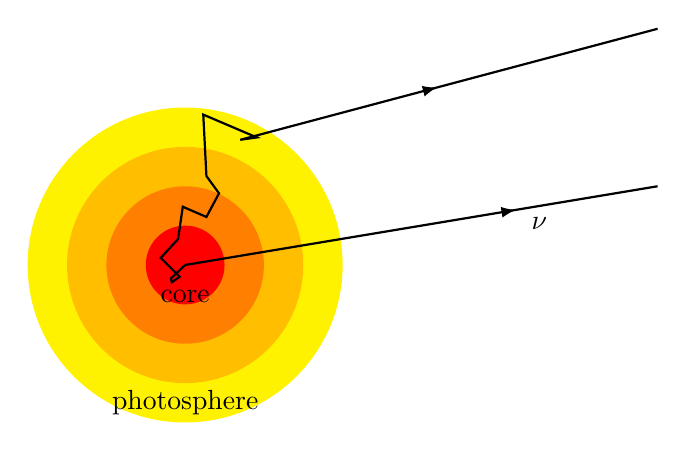
\begin{tikzpicture}[
  particle/.style={thick,decoration={markings, mark=at position .7 with {\arrow[>=latex]{>}}},postaction=decorate}
]
\fill[yellow] (0, 0) circle (2cm);
\fill[orange!50!yellow] (0, 0) circle (1.5cm);
\fill[orange] (0, 0) circle (1cm);
\fill[red] (0, 0) circle (.5cm);

\node at (0, -.4cm) {core};
\node at (0, -1.75cm) {photosphere};

\draw[particle] (0, 0) -- (6cm, 1cm) node[below,near end] {\Pneutrino};
\draw[particle] (0, 0)  -- (-0.18, -0.17)  -- (-0.17, -0.22)  -- (-0.07, -0.15)  -- (-0.31, 0.09)  -- (-0.09, 0.33)  -- (-0.03, 0.74)  -- (0.27, 0.61)  -- (0.43, 0.91)  -- (0.27, 1.13)  -- (0.23, 1.91)  -- (0.91, 1.62)  -- (0.70, 1.59) -- (6cm, 3cm) node[below,near end] {\Pphoton};
\end{tikzpicture}
\caption{Zonsdoorsnede} 
\label{fig:Zonsdoorsnede}
\end{figure}
In \figref{fig:Zonsdoorsnede} zie je een gamma en een neutrino de zon 
verlaten. Beide zijn ongeveer geproduceerd op hetzelfde moment. \\
a. Leg uit dat het neutrino de zon veel sneller zal verlaten dan het gamma.
\begin{center}
    \rule{\textwidth}{0.3mm}\\
    \rule{\textwidth}{0.3mm}\\
\end{center} 
b. Zoek op in BINAS hoe groot het uitgestraald vermogen van de zon is.
\begin{center}
    \rule{\textwidth}{0.3mm}\\
    \rule{\textwidth}{0.3mm}\\
\end{center}
c. Bereken het aantal neutrino's dat de zon per seconde uitzendt.
\begin{center}
    \rule{\textwidth}{0.3mm}\\
    \rule{\textwidth}{0.3mm}\\
    \rule{\textwidth}{0.3mm}\\
    \rule{\textwidth}{0.3mm}\\
    \rule{\textwidth}{0.3mm}\\
\end{center}
d. Bereken de massavermindering van de zon in één jaar.
\begin{center}
    \rule{\textwidth}{0.3mm}\\
    \rule{\textwidth}{0.3mm}\\
    \rule{\textwidth}{0.3mm}\\
    \rule{\textwidth}{0.3mm}\\
\end{center}
Alle neutrino's verlaten de zon. Ze worden naar alle richtingen uitgezonden. 
Op aarde is een neutrinodetector opgesteld met een naar de zon gekeerde 
doorsnede van 5,0 m$^{2}$.\\
e. Zoek op in BINAS hoe groot de afstand van de detector tot de zon gemiddeld 
is. \\
\begin{center}
    \rule{\textwidth}{0.3mm}\\
    \rule{\textwidth}{0.3mm}\\
\end{center}
f. Bereken hoeveel neutrino's per seconde de detector bereiken.
\begin{center}
    \rule{\textwidth}{0.3mm}\\
    \rule{\textwidth}{0.3mm}\\
    \rule{\textwidth}{0.3mm}\\
    \rule{\textwidth}{0.3mm}\\
\end{center}
\bigskip{}

\end{document}
